The ab-initio methods discussed in the previous chapter
are appropriate for systems with a relatively small amount of electrons,
but suffer from cubic time complexity as the number of electrons grows.
If we would like to study systems of molecules, nanoscale structures
or calculate transport coefficients we have to make further approximations
limiting the degrees of freedom of our system.
Instead of solving Schr\"{o}dinger's equation to obtain
the wave function, classical approximations are made to
treat the atoms as point particles, with their interactions
governed by a classical potential. This eliminates both the nucleonic
and electronic degrees of freedom and allows for much larger systems
to be simulated, though at the cost of quantum effects
exhibited by the electrons. In addition, the construction
of molecular dynamics potentials involves guessing at a functional
form, and typically a large amount of parameters to be determined
from experiments and simulations.
In this chapter we will show how quantum mechanics
and classical mechanics can be bridged semi-rigorously,
and also give an introduction to central concepts of molecular dynamics,
such as initialization, integration of the equations of motion
and the construction and evaluation of potentials.

\subsection{From quantum mechanics to molecular dynamics}
This section summarizes the route described in the lecture notes
\parencite[Marx, Dominik and Hutter, J\"{o}rg][pages 1-10]{marx2000}
given at the Winterschool 2000 at the John von Neuman Institute
for Computing, J\"{u}lich.
We will be using SI units as we wish to study the equations of motion
derived from quantum mechanics but in the classical limit.
Our starting point is the full Hamiltonian 
for a set of $N$ electrons and $A$ nuclei:

\begin{equation}
    \begin{split}
        \hat{H}
        &= -\sum_{i=1}^N \frac{\hbar^2}{2m_e} \nabla_i^2
        -\sum_{a=1}^A \frac{\hbar^2}{2M_a} \nabla_a^2
        -\sum_{i=1}^N \sum_{a=1}^A \frac{e^2 Z_a}{R_{ia}} \\
        &+ \sum_{i=1}^N \sum_{j=i+1}^N \frac{e^2}{r_{ij}}
        + \sum_{a=1}^A \sum_{b=a+1}^A \frac{e^2 Z_a Z_b}{R_{ab}}
    \end{split} .
\end{equation}

We want to find solutions to the time-dependent non-relativistic
Schrodinger equation:

\begin{equation}
 i\hbar \frac{\partial}{\partial t} \Psi = \hat{H} \Psi . 
\end{equation}

The wave function is separated in terms of the electronic and nuclear
coordinates with the ansatz:

\begin{equation}
 \Psi \left(\left\{\bm{r}\right\}_i, \left\{\bm{R}\right\}_a, t \right)
    \approx \Phi(\left\{\bm{r}\right\}_i) \chi(\left\{\bm{R}\right\}_a)
    \exp \left[ \frac{i}{\hbar} \int_{t_0}^t
    dt' E_e(t') \right] ,
\end{equation}

with the electronic and nuclear wave functions normalized to unity
at every instance of time. A phase factor is introduced to make
the equations look nice:

\begin{equation}
 E_e = \int d\bm{r} d\bm{R} \Phi^* \chi^* \hat{H} \Phi \chi , 
\end{equation}

where the integration occurs over all spatial coordinates
$\left\{\bm{r}\right\}_i, \left\{\bm{R}\right\}_a$. This is a single determinant
ansatz which must lead to a mean-field description of the dynamics.
Inserting this ansatz into the Schrodinger equation
reveals the following set of equations:

\begin{equation}
 i\hbar \frac{\partial \Phi}{\partial t}
    = -\sum_i \frac{\hbar^2}{2m_e} \nabla_i^2 \Phi
    + \left\{ \int d\bm{R} \chi^* V_{ne} \chi \right\} \Phi , 
\end{equation}

\begin{equation}
 i\hbar \frac{\partial \chi}{\partial t}
    = -\sum_i \frac{\hbar^2}{2M_a} \nabla_a^2 \chi
    + \left\{ \int d\bm{r} \Phi^* \hat{H} \Phi \right\} \chi . 
\end{equation}

These coupled equations form the framework for the
time-dependent self-consistent field (TDSCF) method.
The electrons and nuclei move on a potential energy surface
obtained from averages over the opposite class of
degrees of freedom (the nuclear and electronic wave functions
respectively).
In the framework of classical molecular dynamics
we approximate the nuclei as classical point particles.
This can be done by rewriting the nuclear wave function as

\begin{equation}
 \chi = A \exp[iS/\hbar] , 
\end{equation}

with an amplitude factor $A$ and a phase $S$
which are both considered to be real.
The TDSCF equation for the nuclear wavefunction is rewritten 
in terms of these variables after separating the real
and imaginary parts:

\begin{equation}
 \frac{\partial S}{\partial t} + \sum_a \frac{1}{2M_a}
    (\nabla_a S)^2 + \int d\bm{r} \Phi^* \hat{H} \Phi
    = \hbar^2 \sum_a \frac{1}{2M_a} \frac{\nabla_a^2 A}{A} , 
\end{equation}

\begin{equation}
 \frac{\partial A}{\partial t} + \sum_a \frac{1}{M_a} (\nabla_a A)
    (\nabla_a S) + \sum_a \frac{1}{2M_a} A (\nabla_a^2 S) = 0 . 
\end{equation}

This set of equations is known as the "quantum fluid dynamical representation".
The term for $S$ contains a term for $\hbar$ which vanishes in
the classical limit $\hbar \rightarrow 0$:

\begin{equation}
 \frac{\partial S}{\partial t} + \sum_a \frac{1}{2M_a}
    (\nabla_a S)^2 + \int d\bm{r} \Phi^* \hat{H} \Phi = 0 . 
\end{equation}

This formulation of the nuclear dynamics is isomorphic
to the Hamilton-Jacobi formulation:

\begin{equation}
 \frac{\partial S}{\partial t} + \hat{H} = 0 , 
\end{equation}

with the classical Hamilton function

\begin{equation}
 \hat{H} = T(\left\{P_a\right\}) + V(\left\{R_a\right\}) , 
\end{equation}

with coordinates $\left\{R_a\right\}$ and conjugate momenta 
$\left\{P_a\right\}$.
If we identify the conjugate momenta with the phase $S$ as:

\begin{equation}
 \bm{P}_a = \nabla_a S , 
\end{equation}

we obtain the following Newtonian equations of motion:

\begin{equation}
    \begin{split}
        \frac{d\bm{P}_a}{dt}
    &= -\nabla_a V
    = -\nabla_a \int d\bm{r} \Phi^* \hat{H} \Phi \quad \text{or} \\
        M_a\frac{d^2 \bm{R}_I}{dt^2}
    &= -\nabla_a \int d\bm{r} \Phi^* \hat{H} \Phi \\
    &= -\nabla_a V_e^E \left(\left\{ R_a(t) \right\}\right) .
    \end{split}
\end{equation}

Under this formulation of nuclear dynamics
the nuclei move according to the laws of classical
mechanics in an effective potential $V_e^E$ generated
by the electrons.
After averaging out the electronic degress of freedom
this potential is now only a function of the nuclear coordinates.
For consistency the nuclear wave function appearing
in the TDSCF equation for the electronic
degrees of freedom has to be replaced by the positions
of the nuclei.
This is accomplished by replacing the nuclear density 
$\left| \chi \right|^2$ in the limit $\hbar \rightarrow 0$
by a product of delta functions
$ \prod_a \delta (\bm{R}_a - \bm{R}_a(t)) $ centered
at the instantaneous positions $\left\{ \bm{R}_a(t) \right\}$
of the classical nuclei.
This leads to a time-dependent wave equation
for the electrons:

\begin{equation}
 i\hbar\frac{\partial \Phi}{\partial t} =
    -\sum_i \frac{\hbar}{2m_e} \nabla_i^2 \Phi
    + \hat{V}_{ne} \Phi , 
\end{equation}

which evolve quantum mechanically as the nuclei propagate
classically. This mixed approach is commonly referred to as
\textit{Ehrenfest molecular dynamics}.
Under this formulation of nuclear dynamics the
nuclei evolve classically while the electrons
evolve according to the laws of quantum mechanics.
Although the underlying equations describe a mean-field
theory, the Ehrenfest approach includes transitions
between electronic states.
In order to arrive at a purely classical description of the
dynamics of both the nuclei and the electrons
we need to make further simplifications.
Firstly we restrict the electronic wave function $\Phi$
to the ground state wave function $\Phi_0$
at every instant of time. 
This means the nuclei move on a single potential energy surface:

\begin{equation}
 V_e^E = \int d\bm{r} \Phi_0^* \hat{H} \Phi_0 
    = E_0 \left(\left\{ R_a \right\}\right) , 
\end{equation}

that is obtained by solving the Schrodinger equation
for the ground state electron wave function:

\begin{equation}
 \hat{H} \Phi_0 = E_0 \Phi_0 . 
\end{equation}

Since we are now dealing with a single potential
energy surface, the problem of computing the energy surface
can be decoupled from computing the
expectation values from the electronic wave function.
First one produces an appropriate set of nuclear configurations
by solving the time-independent Schrodinger equation.
Second, these configurations are fitted to an analytical
functional form to produce a global potential energy surface.
Finally the Newtonian equations of motions are solved
on this energy surface, producing a set of classical trajectories.
To deal with the large number of degrees of freedom
as the number of nuclei in the system increases,
the global potential energy surface
is approximated as an expansion of many-body contributions:

\begin{equation}
 V_e^E \approx V_e^{\text{approx}} =
    \sum_a v_1(R_a) + \sum_{a < b} v_2(R_a, R_b)
    + \sum_{a < b < c} v_3(R_a, R_b, R_c) , 
\end{equation}

and is typically truncated at 2, 3 or 4-body interactions
depending on the complexity of the atoms and molecules in the system.
This renders the problem of computing dynamics purely classical:

\begin{equation}
 M_a \frac{d^2 R_a}{dt^2} = -\nabla_a V_e^{\text{approx}} . 
\end{equation}

This reduction in the number of degrees of freedom is a huge simplification
which allows us to study much larger and more complex systems
than ab-initio methods. However, many approximations have to be made
to get to this formulation of atomic/molecular mechanics, and neglecting
the electronic degrees of freedom effectively precludes chemical
transformations from appearing in the simulations.
In addition, the analytical functional forms of the potentials
usually include many parameters to be determined,
and they often have to be tailored to the quantities
one is trying to compute.

\subsection{Molecular dynamics simulations}
The theory in this and the following sections
is based partly on \parencite[Frenkel, Daan
and Smit, Berend][pages 63-107]{frenkel2001understanding},
which explains the physics behind many popular methods 
for computer calculation and simulation.
Classical molecular dynamics is a method
for computing equilibrium and transport properties
of many-body systems obeying classical laws of motion.
While a large number of simplifications have to be made
in order to describe quantum mechanical systems classically,
the approximation works surprisingly well
except for atoms which are quite light ($\text{He}, \text{H}^2$)
or for atoms with a vibrational energy
which is substantially larger than the thermal energy
of the system ($h\nu > k_B T$).
\par
In order to calculate properties of the system
they have to be expressed in terms of the positions
and velocities of the constituent nuclei.
For instance the temperature can be related
to the average kinetic energy of the system:

\begin{equation}
 \langle \frac{1}{2} m v^2 \rangle = \frac{N_f}{2} k_B T , 
\end{equation}

where $N_f$ is the number of degrees of freedom in our system.
At every instant of time the total kinetic energy
of our system defines an instantaneous temperature,
which has to averaged over a large number of timesteps
in order to produce the equilibrium property.
In practice, one is satisfied when the fluctuations
in the instantaneous temperature appear reasonably small.
\par
To run a molecular dynamics simulation one requires
a set of initial conditions, i.e. a set of initial positions and velocities
for every atom in the system. Typically the atoms
are placed by replicating a unit cells a number of times
in every dimension. A unit cell consists of a set
of lattice vectors which define the placement of every atom in the
unit cell. For instance the face-centered cubic cell (FCC)
contains 4 atoms:

\begin{equation}
    \begin{split}
        \bm{r}_1 &= (0, 0, 0) \\
        \bm{r}_2 &= (\frac{b}{2}, \frac{b}{2}, 0) \\
        \bm{r}_3 &= (0, \frac{b}{2}, \frac{b}{2}) \\
        \bm{r}_4 &= (\frac{b}{2}, 0, \frac{b}{2}) , \\
    \end{split}
\end{equation}

where $b$ is known as the lattice constant and defines
the size of the unit cells.
In figure \ref{fig:md} we have an image of a
box of atoms visualized using the Visual Molecular Dynamics (VMD\footnote
{\href{https://www.ks.uiuc.edu/Research/vmd/}{Visual Molecular Dynamics (VMD)}}) software.
In this system we have a group of water molecules over a Self-Assembled
Monolayer (SAM) surface, consisting of C12 molecules attached to a 
sulfhydryl group. In this case the SAM surface is placed regularly
while the water molecules are placed randomly, ensuring no molecules are too close.

\begin{figure}[H]
    \centering
    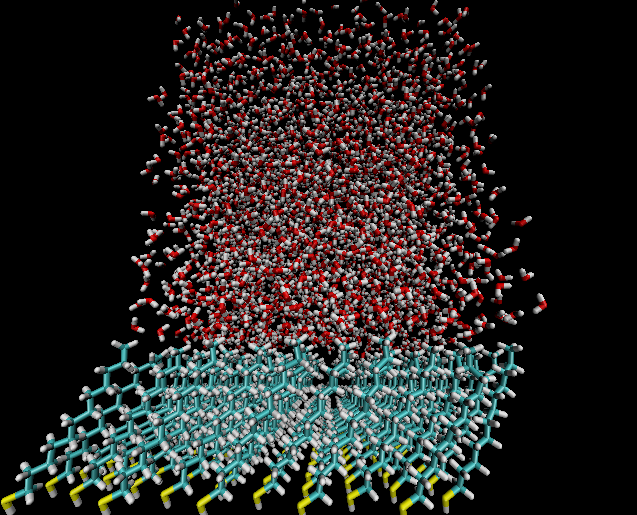
\includegraphics[width=\textwidth]{md.png}
    \caption{Water molecules over a SAM surface. Hydrogen atoms in white,
        oxygen in red, carbon in blue and sulfur in yellow.}
    \label{fig:md}
\end{figure}

\par
The velocities are typically initialized with a random uniform
distribution or the Maxwell-Boltzmann distribution.
The Maxwell-Boltzmann distribution is the one most often used,
since the equilibrium distribution tends towards this distribution.
The exact form however will differ from the one we started with.
\par
Given these initial conditions, the system will not be in an
equilibrium state at $t=0$. To evolve the system
to an equilibrium state one most commonly advances the system in time
until fluctuations in dynamic
properties such as the total potential energy or the temperature
settle down. Once we are in equilibrium we can start calculating
thermodynamic averages.
\newline
\newline
As we mentioned before, the global energy surface
as a function of nuclear coordinates $\left\{ \bm{r} \right\}$
is approximated as an expansion of many-body contributions:

\begin{equation}
 V_e^E \left(\left\{ \bm{r} \right\}\right) =
    \sum_i v_1(r_i) + \sum_{i < j} v_2(r_i, r_j)
    + \sum_{i < j < k} v_3(r_i, r_j, r_k) , 
\end{equation}

wherein each $N$-body term is an analytical function
of $N$ coordinates.
As an atom moves on the energy surface
it feels a force which is the gradient of the potential energy surface.
This means atom $i$ feels an acceleration:

\begin{equation}
 \bm{F}_i = m_i \frac{d^2 \bm{r}_i}{dt^2} =
    -\nabla_i V_e^E \left( \left\{ \bm{r} \right\}\right) . 
\end{equation}

For a system of $N$ atoms with only pairwise interactions
this means the forces must be calculated $N(N-1)/2$ times
for every timestep which means we have a time complexity
of order $\mathcal{O}(N^2)$. The force calculation is by far
the most important part of any molecular dynamics simulation,
and the most time consuming.
A number of techniques are employed in order to reduce
the time usage, perhaps the most common is the use of neighbor
lists. Using neighbor lists, each atom carries a list of neighbors
within a cut-off radius $r_{cut}$ and interactions
beyond this cut-off are neglected.
This reduces the time-complexity to merely
$\mathcal{O}(N)$, with a proportionality constant
dependent upon the average number of neighbors in the system
within a cutoff $r_{cut}$. For a large system this can be a
huge reduction in complexity, but the choice of cut-off
can obviously massively impact the dynamics of the system.
\par
In order to simulate the dynamics of a system governed by
a conservative force $\bm{F} = - \nabla V_e^E$
we need to integrate the Newtonian equations of motion.
The equations of motion are typically not solvable
analytically, which means we require an effective numerical
method for integration. Some important considerations
for molecular dynamics are conservation of energy
and accuracy for large time steps.
The most common method used is the Velocity-Verlet algorithm.
At any given time step $t$, the position $\bm{r}(t + \Delta t)$
and velocity $\bm{v}(t + \Delta t)$ at the next time step
$t + \Delta t$ is calculated as:

\begin{equation}
    \begin{split}
        \bm{r}(t + \Delta t)
        &= \bm{r}(t) + \bm{v}(t) \Delta t
        + \frac{1}{2} \bm{a}(t)\Delta t^2 , \\
        \bm{a}(t + \Delta t)
        &= -\frac{1}{m} \nabla V_e^E(\bm{r}(t + \Delta t)) , \\
        \bm{v}(t + \Delta t)
        &= \bm{v}(t) + \frac{1}{2}
        (\bm{a}(t) + \bm{a}(t + \Delta t)) \Delta t .
    \end{split}
\end{equation}

The error in the Velocity-Verlet method is of order
$\mathcal{O}(\Delta t^2)$, which means that it is
not particularly accurate for large time steps
over a long time. However, the long term
energy drift of the method is small, which is very desirable.
It is also not very memory-intensive, which matters
for simulating very large systems.
\newline
\newline
Molecular dynamics is usually performed within
a cubic box of fixed volume $V = L_x \cdot L_y \cdot L_z$,
where $L_i$ is the length of the box in direction $i$.
Molecular dynamics is typically limited by the number
of particles we are able to simulate, of the order
$10^6 - 10^8$, which means the size of the box
is often decided by the desired density $\rho = N / V$.
Since the number of particles is always much smaller
than the number of particles in realistic systems,
approximations are required. Periodic boundary conditions
can be applied to the box in order to approximate
an infinite system. Typically particle coordinates are restricted
to the simulation box, which can be expressed in pseudocode as:

\begin{algorithm}[H]
\caption{Continuity}
    \begin{algorithmic}
        \If{$x < -L_x / 2$}
            \State{$x \mathrel{+}= L_x$}
        \EndIf
        \If{$x > L_x / 2$}
            \State{$x \mathrel{-}= L_x$}
        \EndIf
    \end{algorithmic}
\end{algorithm}

Distance and distance vectors between particles
should also obey the minimum image convention:

\begin{algorithm}[H]
\caption{Minimum image}
    \begin{algorithmic}
        \State $dx = x_j - x_i$
        \If{$dx < -L_x / 2$}
            \State{$dx \mathrel{+}= L_x$}
        \EndIf
        \If{$dx > L_x / 2$}
            \State{$dx \mathrel{-}= L_x$}
        \EndIf
    \end{algorithmic}
\end{algorithm}

These conditions should be applied in every dimension.
This approach runs the risk of introducing nonphysical artifacts
of the simulation, such as a macromolecule interacting with its own image,
and for coulombic interactions the system must be charge neutral to avoid
summing to an infinite charge.
The optimal system size with periodic boundary conditions
will therefore depend on the intended simulation length, the desired accuracy
and the dynamics which are being studied.
\newline
\newline
Thus far we have discussed molecular dynamics for a system of $N$ particles
within a fixed volume $V$ and constant energy $E$, i.e. in the
microcanonical ensemble NVE. Other ensembles are also possible,
such as the canonical ensemble NVT and the isothermal-isobaric ensemble
NPT.
\par
Simulations in the canonical ensemble can be achieved by modifying the Verlet
integration algorithm. The simplest thermostat possible
follows from the equipartion theorem (see for example \cite{equipart}):

\begin{equation}
 T \propto \langle mv^2 \rangle , 
\end{equation}

meaning some amount of kinetic energy i.e. velocity
can be added or subtracted to every atom in order to maintain
a constant temperature at every timestep.
Multiplying every velocity by a factor $\lambda = \sqrt{T_0 / T(t)}$
where $T(t)$ is the instantaneous temperature and $T_0$
is the desired temperature will achieve the desired effect.
This approach significantly alters the trajectories of the system however,
which means this thermostat should only be applied for adjusting
the temperature of the system and not for taking ensemble averages
in equilibrium.
\par
The most common thermostat used is the Nosé-Hoover thermostat,
which is one of the most accurate and efficient algorithms
for achieving realistic constant-temperature conditions
(see the lecture notes \parencite[Shell, M. Scott]{che210D2012}).
Nosé introduced an extended Hamiltonian with two additional degrees of freedom:

\begin{itemize}
    \item $s$ - the position of an imaginary coupled heat reservoir
    \item $p_s$ - the conjugate momentum of the heat reservoir
\end{itemize}

In addition it introduces an effective mass $Q$ such that $p_s = Q\frac{ds}{dt}$.
\par
Hoover modified Nosé's approach by introducing the Hamiltonian:

\begin{equation}
 H = \frac{1}{2} \sum m_i \left| \bm{p}_i \right|^2 + U(\bm{r}) + \frac{\xi Q}{2}
    + 3Nk_B T \ln{s} , 
\end{equation}

where $\xi$ is a friction coefficient and $\bm{p}_i = m_i\bm{v}_i \times s$
are the particle momenta. This leads to a new set of Newtonian equations of motions
with an additional force that is proportional to the velocity:

\begin{equation}
\begin{split}
    \frac{d\bm{r}_i}{dt} &= \bm{v}_i \\
    \frac{d\bm{v}_i}{dt} &= - \frac{1}{m_i} \frac{\partial U(\bm{r})}{\partial \bm{r}_i}
    - \xi \bm{v}_i \\
    \frac{d\xi}{dt} &= \left( \sum m_i \left| \bm{v}_i \right|^2 - 3Nk_b T \right) / Q \\
    \frac{d \ln{s}}{dt} &= \xi .
\end{split}
\end{equation}

These can then be solved with a numerical integration scheme such as the
velocity-Verlet algorithm.

\subsection{Molecular dynamics potentials}
The dynamics of an ensemble of particles is governed by
their interactions. In molecular dynamics we stipulate that
the interactions are decided only by the relative positions
of the particles, i.e. only conservative forces act on the atoms.
This means that the force on atom $i$ is fully described
by a potential energy $U$:

\begin{equation}
 \bm{F}_i = -\nabla_i U \left(\left\{ \bm{r} \right\} \right) , 
\end{equation}

which in principle depends on the position of atom $i$
and all other atoms in the system. Finding an appropriate potential
for the system of atoms which you intend to study can be ardous work,
and usually involves fitting an analytical functional form
with a large set of parameters to a potential energy surface
from ab initio quantum mechanical calculations.
\par
Potentials can be classified as either bonded or non-bonded.
Bonded potentials compute the interactions for a predefined
set of atoms and molecules in the simulations, while
non-bonded potentials compute the interactions
between \textit{all} pairs, triplets etc. of atoms
(usually within a certain radius).
Larger, more complex systems typically contain a mix of
bonded and non-bonded potentials, for example a system of rigid water molecules
interacting with a surface of carbon atoms.
\par
One of the simplest potentials meant to simulate a realistic system
is the Lennard-Jones potential:

\begin{equation}
 U(r_{ij}) = 4\epsilon \left(\left(\frac{\sigma}{r_{ij}}\right)^{12}
    - \left(\frac{\sigma}{r_{ij}}\right)^{6}\right) , 
\end{equation}

with $r_{ij} = \left| \bm{r}_j - \bm{r}_i \right|$.
For the Lennard-Jones potential there are only two parameters to be decided,
a characteristic energy $\epsilon$ and a characteristic length $\sigma$.
This potential is meant to emulate the relatively weak interactions
between noble gas atoms such as Argon.
It can be separated into two terms:

\begin{itemize}
    \item $\mathrel{-} \left(\frac{\sigma}{r}\right)^6$ - owing to the long-term
        attraction from van der Waals interactions
    \item $\mathrel{+} \left(\frac{\sigma}{r}\right)^{12}$ - owing to the short-term repulsion
        from the Pauli principle
\end{itemize}

While the van der Waals term is justified by theory, the repulsion term
is justified by numerical efficiency - as it contains the square of the van der Waals
term - and because it models the Pauli repulsion accurately.
In figure \ref{fig:lennard-jones} we have plotted the Lennard-Jones potential
as a function of interatomic distance.
This form of the potential, with close repulsion and distant attraction
is very common among molecular dynamics potentials, though often with
modifications.

\begin{figure}[H]
    \centering
    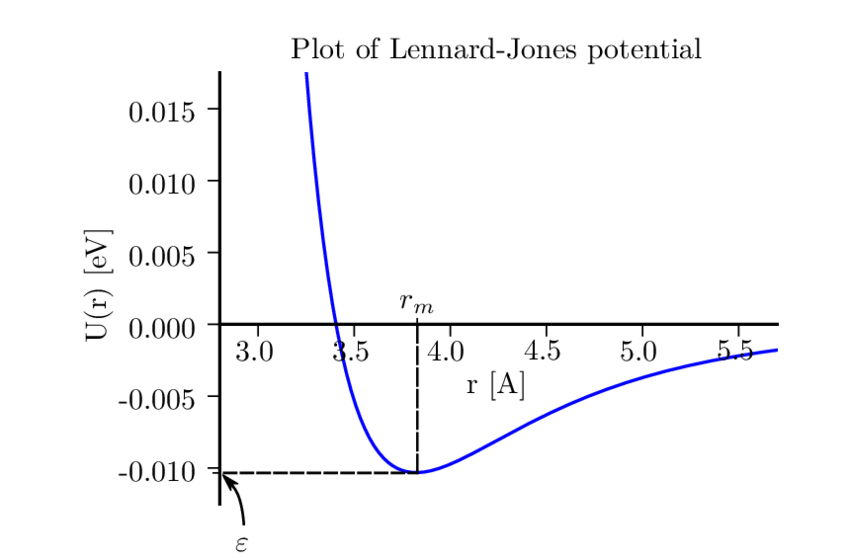
\includegraphics[width=\textwidth]{lennard_jones.png}
    \caption{Lennard-Jones potential as a function of interatomic distance.
        Units in Angstrom and electronvolts.
        Reprinted from \parencite[Molecular dynamics modelling of clay-fluid interfaces]
            {phdthesis}.}
    \label{fig:lennard-jones}
\end{figure}

\par
While the Lennard-Jones potential is very simple, requiring only two parameters
to be determined, it has shown to be effective at modelling noble gas atoms
and is commonly used as a building block for more complicated interactions.
\par
Another simple and common potential is the Stillinger-Weber potential,
which is meant to model the interactions between silicon atoms
(see the lecture notes \parencite[Abrams, Cameron]{che8002013}).
Silicon forms tetrahedral bonded structures as well as pairwise interactions
which means the potential includes a twobody and a threebody interaction:

\begin{equation}
    U = \sum_{i < j} v_2(r_{ij}) + \sum_{i < j < k} v_3(\bm{r}_i, \bm{r}_j, \bm{r}_k) .
\end{equation}

The twobody interaction models the pairwise interaction:

\begin{equation}
    v_2(r) =
    \begin{cases}
        \epsilon A (Br^{-p} - r^{-q}) \exp \left[ (r - a)^{-1} \right],
        & r < a \\
        0 & r \geq a
    \end{cases}
\end{equation}

This twobody term resembles the Lennard-Jones potential,
but with an exponential cutoff.
The threebody term models the tetrahedral angles,
and is a sum over three triplets:

\begin{equation}
    v_3(\bm{r}_i, \bm{r}_j, \bm{r}_k) = h_{jik} + h_{ijk} + h_{ikj} ,
\end{equation}

with the angular interaction $h_{jik} = h(r_{ij}, r_{ik}, \theta_{jik})$ and

\begin{equation}
    h_{jik} =
    \begin{cases}
        \displaystyle\epsilon \lambda \exp \left[ \frac{\gamma}{r_{ij} - a}
        + \frac{\gamma}{r_{ik} - a} \right]
        \left(\cos{\theta_{jik}} - \cos{\theta_{jik}^0} \right)^2 & r_{ij} < a \\[10pt]
        \displaystyle 0 & r_{ij} \geq a
    \end{cases}
\end{equation}

where $\theta_{jik}^0$ is an "equilibrium" angle.
The terms $\epsilon, A, B, p, q, \lambda, \gamma$ are parameters
to be decided and $a$ is a cutoff radius.
The inclusion of the threebody terms prove to be quite important
in silicon maintaining its equilibrium crystal structure.
The Stillinger-Weber potential agrees quite well with experiment,
and its relatively simple form makes it well suited for
the testing and evaluation of new potentials.
\par
A more complicated set of potentials is the Effective Medium Theory (EMT)
family of potentials, developed to describe the late transition
metals in the FCC crystal structure. The potential was first
described by \parencite[Jacobsen, K.W.; Nørskov, J.K. and
Puska, M.J.]{jacobsen1987interatomic}, but the most common set of parameters
was published in the later article by \parencite[Jacobsen, K.W.;
Stoltze, P. and Nørskov, J.K.]{jacobsen1996semi}.
These potentials are based on the effective medium theory concept
of an electron density with a volume-dependent contribution to
the total energy.
Effective Medium Theory computes the energy of an atom in an
arbitrary environment by computing it first in a reference system
and then estimating the energy difference between the real system
and the reference system.
The total energy is written as:

\begin{equation}
    E = \sum_i E_{c,i} + \left( E - \sum_i E_{c,i} \right) ,
\end{equation}

where $E_{c,i}$ is the energy of atom $i$ in the reference system.
The correction $E - \sum_i E_{c,i}$ is made small enough so that
it can be estimated using approximate methods such as perturbation theory.
From Density Functional Theory the total energy can be written as:

\begin{equation}
    E = \sum_i E_{c,i}(n_i) + \Delta E_{AS} + \Delta E_{\text{1el}} ,
\end{equation}

where $E_c$, $\Delta E_{AS}$ and $\Delta E_{\text{1el}}$ are known as
the cohesive function, atomic-sphere correction and one-electron correction
respectively. The density argument $n_i$ is known as the embedding density,
which connects the surroundings of atom $i$ to the reference system 
of atom $i$. The atomic-sphere correction is the difference in
electrostatic and exchange-correlation energy for the atoms in the system
of interest and the reference system.
The one-electron correction is the sum of one-electron energies in the two
systems. If the one-electron correction is small and can be neglected
a pair-potential approximation leads to the expression:

\begin{equation}
    \begin{split}
    E   &=\sum_i \left[ E_{c,i}(n_i) + \Delta E_{AS} \right] \\
        &= \sum_i \left\{E_{c,i}(n_i) + \frac{1}{2} \left[
        \sum_{j \neq i} V_{ij}(r_{ij}) - \sum_{j \neq i}^{\text{ref}}
        V_{ij}(r_{ij}) \right] \right\} .
    \end{split}
\end{equation}

The one-electron correction is often not small, so this is usually
referred to as just the atomic-sphere correction.
The embedding density $n_i$ is computed by superimposing
density contributions from the neighboring atoms:

\begin{equation}
    n_i = \sum_{j \neq i} \Delta n_j(s_i, r_{ij}) ,
\end{equation}

where the density tail $\Delta n (s, r)$ from a neighboring
atom a distance $r$ averaged over a sphere of radius $s$
has an exponential form:

\begin{equation}
    \Delta n(s,r) = \Delta n_0 \exp \left[ \eta_1 (s - s_0)
    - \eta_2 (r - \beta s_0) \right] .
\end{equation}

The size of the sphere $s$ is chosen so that the total charge
within in zero. 
The geometric factor $\beta = \left(16\pi / 3\right)^{1/3} / \sqrt{2}$
is related to the nearest-neighbor distance $d_{nn} = \beta s$.
For this set of electron densities
there is a one-to-one correspondence between the average electron
density and its neutral-sphere radius.
This relationship has been shown to be approximately exponential:

\begin{equation}
    \bar{n}(s) = n_0 \exp \left[ - \eta(s - s_0) \right] .
\end{equation}

For an FCC crystal of varying nearest-neighbor distance
$r = \beta s$ the neutral-sphere radius can be expressed as:

\begin{equation}
    s_i = s_0 - \frac{1}{\beta \eta_2} \log \left(
    \frac{\sigma_{1,i}}{12} \right) ,
\end{equation}

where

\begin{equation}
    \sigma_{1, i} = \sum_{j \neq i} \exp \left[ - \eta_2
    \left( r_{ij} - \beta s_0 \right) \right] .
\end{equation}

The cohesive function is parameterized as a function
of the neutral-sphere radius using the functional form:

\begin{equation}
    \begin{split}
        E_c (s) &= E_0 f\left[ \lambda \left( s - s_0 \right) \right], \\
        f\left( x \right) &= \left( 1 + x \right) \exp \left( - x \right)
    \end{split}
\end{equation}

where $s_0$ is the equilibrium (zero pressure) neutral-sphere radius.
Finally the atomic sphere correction is written as:

\begin{equation}
    \Delta E_{AS}(i) = \frac{1}{2} \left[ \sum_{j \neq i} V(r_{ij})
    - 12 V(\beta s_i) \right],
\end{equation}

where the factor 12 comes from the 12 nearest neighbors at
a distance $r = \beta s_i$ in the FCC reference system.
The pair potential is parameterized as:

\begin{equation}
    V(r) = - V_0 \exp \left[ - \kappa \left( r/\beta - s_0 \right) \right] .
\end{equation}

This has been found to give reasonable descriptions
of the six fcc metals Cu, Ag, Au, Ni, Pd, Pt and their alloys.
Further description and parameters can be found in the article
\parencite[Jacobsen, K.W.;
Stoltze, P. and Nørskov, J.K.]{jacobsen1996semi}.
